\newpage
\subsection{Caso d'uso UC6:  Ricerca API }
\label{UC6}
\begin{figure}[ht]
	\centering
	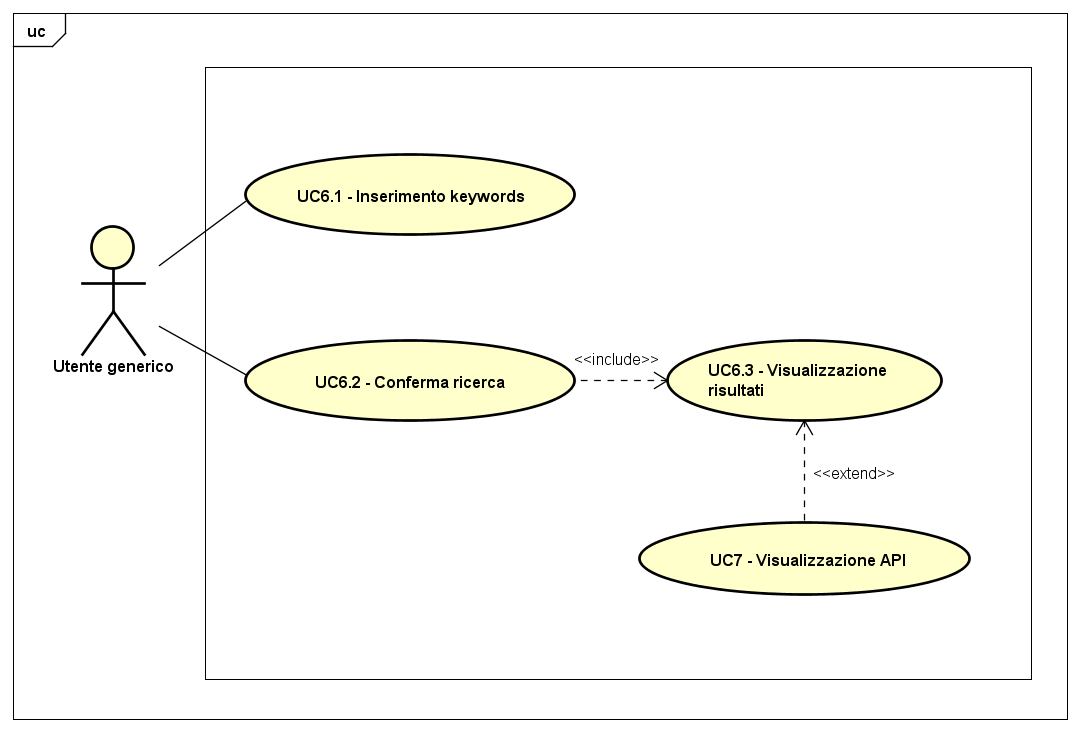
\includegraphics[scale=0.45]{UML/UC6.png}
	\caption{UC6: Ricerca API }
\end{figure}

\begin{longtable}{ l | p{11cm}}
	\hline
	\rowcolor{Gray}
	 \multicolumn{2}{c}{UC6 - Ricerca API} \\
	 \hline
	\textbf{Attori} & Utente Non Autenticato, Utente Autenticato \\
	\textbf{Descrizione} & L'utente non autenticato inserisce i dati necessari alla sua ricerca di API. L'utente autenticato, oltre alle funzionalità offerte all'utente non autenticato, può filtrare la ricerca affinchè includa o escluda le proprie API \\
	\textbf{Pre-Condizioni} & L'utente ha scelto di effettuare la ricerca di API \\
	\textbf{Post-Condizioni} & L'utente ha effettuato la ricerca di API e ne ha visualizzato il risultato, oppure la procedura è fallita \\
	\textbf{Scenario Principale} & 
	\begin{enumerate*}[label=(\arabic*.),itemjoin={\newline}]
		\item L'utente può inserire il nome di API (UC6.1)
		\item L'utente può inserire il nome di un utente (UC6.2)
		\item L'utente può scegliere una categoria di ricerca (UC6.3)
		\item L'utente può confermare i dati inseriti (UC6.4) e visualizzare i risultati forniti dall'applicazione web (UC6.5)
	\end{enumerate*}\\
	\textbf{Scenari Alternativi} & 
	\begin{enumerate*}[label=(\arabic*.),itemjoin={\newline}]
		\item L'utente visualizza un errore e la ricerca non ritorna alcun risultato (UC6.6) 
	\end{enumerate*}\\
\end{longtable}